\section{连通与分隔}
\label{sec:graph-connectivity-separation}

上一节的可达关系一次只回答两个顶点之间的问题。道路网规划还需要整体的回答：全部城市分成几片互相到达的区域，封闭哪些路口或道路会把区域切开。本节先用可达关系把顶点集划分为连通分量，再对有向图区分强、弱两种连通，最后研究删除顶点或边怎样改变连接。这里只讨论结构上的路径是否存在，不涉及概率中的条件独立；后者有自己的分离判据，留到后续关于推断的部分。

\subsection{无向图的连通分量}
\label{sec:graph-conn-components}

在无向图中，可达关系是等价关系（第~\ref{sec:graph-conn-reachability}小节）。由定理~\ref{thm:sets-equivalence-partition}，它的等价类构成顶点集的一个划分。

\begin{definition}[连通分量]
\label{def:graph-conn-component}
无向图$\mathcal G=(V,E)$中可达关系的每个等价类$C\subseteq V$称为$\mathcal G$的一个\term{连通分量}（connected component）；有时也把诱导子图$\mathcal G[C]$称为连通分量。若$\mathcal G$非空且恰有一个连通分量，即任意两个顶点之间都有路径，就称$\mathcal G$是\term{连通}（connected）的。
\end{definition}

这个划分有三条直接的性质。第一，同一分量中任意两点可达，而且连接它们的路径不会离开该分量，因为路径上的每个顶点都与起点可达；所以$\mathcal G[C]$本身是连通图。第二，不同分量之间没有边：若$i\in C$、$j\in C'$之间有边，则$j$从$i$可达，二者应属同一分量。第三，划分由图唯一确定，因为等价类只取决于可达关系本身，与我们从哪个顶点开始寻找无关。

图~\ref{fig:graph-conn-components}(a)是三角形$\{1,2,3\}$加上孤立顶点$4$。$4$没有邻居，只与自身可达，单独构成一个分量，所以这张图有两个分量$\{1,2,3\}$与$\{4\}$，不连通。对顶点集为空的图，可达关系没有等价类，分量数为$0$；按定义它不算连通图。凡是用“恰有一个分量”判断连通性的论证，都需要先排除这个边界情形。

\begin{figure}[!htb]
  \centering
  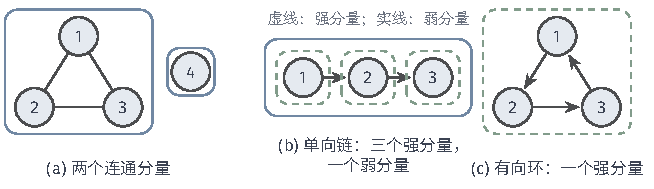
\includegraphics[width=110.808mm]{figures/01-basic-mathematics/04-graphs/tikz/c1-components/figure.pdf}
  \caption{连通分量。蓝色实线框是无向图或底层无向图的连通分量，绿色虚线框是强连通分量。(a)孤立点自成一个分量；(b)单向链$1\to2\to3$忽略方向后连成一片，但没有两个顶点能互相到达，每个顶点自成一个强分量；(c)有向环上任意两个顶点都能互相到达，三个顶点属于同一个强分量。}
  \label{fig:graph-conn-components}
\end{figure}

\paragraph{删除边与替代路径}
连通性取决于是否还有替代路径，而不只取决于边的数目。在贯穿图中删除边$\{2,3\}$，$2$与$3$仍可经$1$或$4$相连，图依然连通；在图~\ref{fig:graph-conn-cut-bridge}(a)中删除连接两个三角形的边$\{3,4\}$，两侧之间就再没有路径，图分成两个分量。两次都只删除了一条边，结果不同的原因是前者的边位于环上，环的另一侧提供了替代路径。第~\ref{sec:graph-conn-separators}小节会把这一观察写成桥的判别条件。

\subsection{强连通与弱连通}
\label{sec:graph-conn-strong-weak}

有向图中可达不对称，“$j$从$i$可达”不能像无向图那样直接用来划分顶点。有两种自然的修补：要求双向都可达，或者干脆忽略方向。

\paragraph{强连通分量}
若$j$从$i$可达且$i$从$j$可达，称$i,j$相互可达。相互可达关系是自反的（零长度行走）、对称的（定义本身对$i,j$对称）、传递的（两个方向分别把行走首尾相接），因此是等价关系。它的等价类称为\term{强连通分量}（strongly connected component）；若有向图非空且只有一个强连通分量，即任意有序顶点对$(i,j)$之间都有从$i$到$j$的有向路径，就称它\term{强连通}（strongly connected）。

图~\ref{fig:graph-conn-components}(b)的单向链中，$1$能到$3$而$3$不能到$1$，任何两个不同顶点都不相互可达，所以三个顶点各自构成一个强分量。(c)的有向环中，从任一顶点出发沿环走一段就能到达其他任一顶点，三个顶点同属一个强分量，图是强连通的。可见强分量把“绕得回来”的顶点归在一起；把单向可达的顶点合进同一个强分量是错误的。

\paragraph{弱连通分量}
忽略方向后，用底层无向图（第~\ref{sec:graph-conn-directions}小节）的连通分量来划分顶点，所得的分量称为原图的\term{弱连通分量}（weakly connected component）；底层无向图连通时，称原有向图\term{弱连通}（weakly connected）。图~\ref{fig:graph-conn-components}(b)的单向链去掉箭头后是一条路径，只有一个弱分量。

两种分量的关系是单向的。每条有向路径去掉箭头后都是底层无向图中的路径，所以相互可达的两个顶点必在同一个弱分量中：每个强分量都包含在某个弱分量之内，强连通蕴含弱连通。反过来不成立，单向链弱连通但不强连通，其中$3$到不了$1$。所以弱连通只说明忽略方向后连成一片，不保证任何两个顶点能双向到达。怎样在线性时间内求出全部强分量，是第~\ref{sec:graph-connectivity-computation}节的内容。

\subsection{分隔集、割点与桥}
\label{sec:graph-conn-separators}

连通分量描述的是现状；规划者还关心脆弱性：封闭哪些路口能把两个区域隔开，哪个单独的路口或哪条单独的道路一旦失效就会让网络断开。

\paragraph{分隔集}
要把两组顶点隔开，就要删除一些别的顶点，使两组之间不再有路径。被删除的顶点不能属于要隔开的两组本身。

\begin{definition}[分隔]
\label{def:graph-conn-separation}
设$A,B,S\subseteq V$两两不相交。若在$\mathcal G-S$中不存在从$A$中顶点到$B$中顶点的路径，就称$S$\term{分隔}（separate）$A$与$B$，称$S$为$A$与$B$之间的一个\term{分隔集}（separator）。
\end{definition}

等价地，$\mathcal G$中从$A$到$B$的每条路径都至少经过$S$中的一个顶点：若某条路径避开了$S$，它在$\mathcal G-S$中仍然存在。这个等价说法提醒我们，验证一个候选集要检查全部路径，找到一条被阻断的路径并不够。

在图~\ref{fig:graph-conn-separator-sets}中取$A=\{1\}$、$B=\{4\}$。候选集$S=\{2\}$阻断了路径$(1,2,4)$，但$\mathcal G-\{2\}$中仍有路径$(1,3,4)$，所以$\{2\}$不分隔$1$与$4$；删除$S=\{2,3\}$后，$1$的邻居全部被删除，$1$与$4$之间不再有路径，$\{2,3\}$才是分隔集。若$A$与$B$在原图中已经位于不同分量，空集就分隔它们，因为不删除任何顶点时本来就没有路径。

\begin{figure}[!htb]
  \centering
  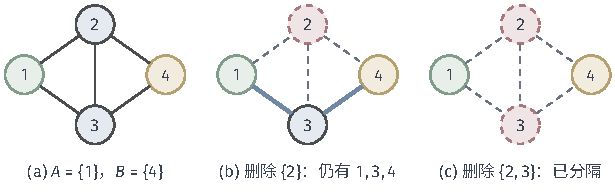
\includegraphics[width=104.186mm]{figures/01-basic-mathematics/04-graphs/tikz/c1-separator-sets/figure.pdf}
  \caption{在贯穿图中检验分隔集，$A=\{1\}$为绿色，$B=\{4\}$为黄色，被删除的候选集$S$为红色虚线顶点。(b)删除$\{2\}$后蓝色路径$(1,3,4)$仍然存在，$\{2\}$不是分隔集；(c)删除$\{2,3\}$后从$1$到$4$没有路径，$\{2,3\}$分隔$\{1\}$与$\{4\}$。}
  \label{fig:graph-conn-separator-sets}
\end{figure}

不指定$A,B$时，也可以只问删除一组顶点后图是否断开。对连通图$\mathcal G$，若$\mathcal G-S$不连通，则$S$分隔$\mathcal G-S$中任意两个不同分量的顶点集。例如贯穿图删除$\{2,3\}$后余下$\{1\}$与$\{4\}$两个分量。第~\ref{sec:graph-separator-blocks}节将沿这样的分隔集把图分成可以分别处理的块。

\paragraph{割点与桥}
最脆弱的情形是只删除一个顶点或一条边就增加了分量数。删除顶点$v$后$\mathcal G-\{v\}$的分量数大于$\mathcal G$的分量数，称$v$为\term{割点}（cut vertex）；删除边$e$后$\mathcal G-e$的分量数大于$\mathcal G$的分量数，称$e$为\term{桥}（bridge）。

图~\ref{fig:graph-conn-cut-bridge}(a)由两个三角形和连接它们的边$\{3,4\}$组成。删除$3$后，$\{1,2\}$与$\{4,5,6\}$分开，$4$同理，所以$3,4$是割点；删除边$\{3,4\}$也把两侧分开，它是桥。三角形内部的边都不是桥，三角形顶点$1,2,5,6$也不是割点。(b)的链中，中间顶点$2$是割点，两条边都是桥；(c)的三角形中，删除任意一个顶点或一条边，剩下的部分仍然连通。

\begin{figure}[!htb]
  \centering
  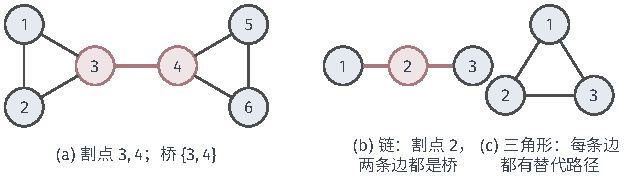
\includegraphics[width=106.765mm]{figures/01-basic-mathematics/04-graphs/tikz/c1-cut-vertex-bridge/figure.pdf}
  \caption{割点与桥，红色顶点为割点，红色粗边为桥。(a)两个三角形由一条边相连，这条边是桥，它的两个端点是割点；(b)链上每条边都是桥，中间顶点是割点，端点$1,3$虽是桥的端点却不是割点；(c)三角形的每条边都位于环上，删除任何一条边或一个顶点都不会断开。}
  \label{fig:graph-conn-cut-bridge}
\end{figure}

\paragraph{为什么边位于环上就不是桥}
设$e=\{i,j\}$。删除$e$只可能拆开$e$所在的那个分量$C$：$C$中任一顶点$x$在原图中有到$i$的路径，若这条路径不经过$e$，删除后它仍连到$i$；若经过$e$，取它第一次到达$i$或$j$之前的部分，删除后$x$仍连到$i$或$j$。所以$\mathcal G-e$中$C$至多分成$i$所在和$j$所在两部分，分量数至多增加$1$。由此得到判别条件：$e$是桥，当且仅当$\mathcal G-e$中没有从$i$到$j$的路径。

若$e$位于某个环上，沿环的另一侧就是$\mathcal G-e$中从$i$到$j$的路径，$e$不是桥。反过来，若$\mathcal G-e$中有从$i$到$j$的路径$P$，它不经过$e$，长度至少为$2$，接上$e$就得到一个环。所以一条边是桥，当且仅当它不在任何环上。这正是图~\ref{fig:graph-conn-cut-bridge}中三角形与链的区别。

\paragraph{顶点分隔与边分隔不同}
删除一个顶点会同时删除它的全部邻边，可能把分量拆成很多块：在一个中心顶点与其余每个顶点各连一条边的星形图中，删除中心顶点后，其余每个顶点都自成一个分量。删除一条边却如上所述至多增加一个分量。此外，桥的端点不一定是割点，例如图~\ref{fig:graph-conn-cut-bridge}(b)的端点$1$；没有桥的图也可能有割点，例如两个三角形共用一个顶点时，共用的顶点是割点，而每条边都在某个三角形上。所以“删点能否断开”与“删边能否断开”需要分别检查。
